\changecolours{ScoutGreen}
\section[Otimização de Consultas]{Princípios e Heurísticas de Otimização de Consultas}

% ------------------------------------------------------------------------------
\twocolframe[title={O Pipeline de Processamento de Consultas no SGBD},leftcol=6.8cm,rightcol=7.2cm]{%
  \alert{As Fases Internas do Motor de BD}\par
  \itemseps[topsepi=0.5mm,itemsepi=1mm,labelsep=2mm,leftmargini=3mm]
  \begin{enumerate}
    \item \textbf{Parser:} Análise léxica, sintática e semântica do SQL contra o catálogo.
    \item \textbf{Árvore Canônica:} Representação algébrica literal da consulta.
    \item \textbf{Otimizador Lógico:} Aplica equivalências algébricas e heurísticas de reordenação.
    \item \textbf{Otimizador Físico:} Escolhe algoritmos de acesso (Hash, B-Tree, Nested Loop) com base em estatísticas.
    \item \textbf{Execução:} Geração de código e leitura em disco.
  \end{enumerate}
}{%
  \alert{Fluxo de Otimização}\par
  \vspace{0.2cm}
  \centering
  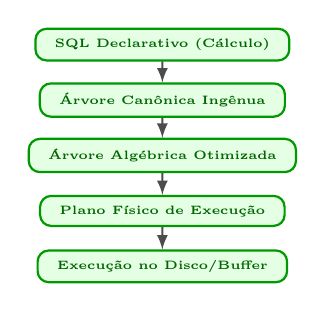
\begin{tikzpicture}[
    scale=0.88,
    every node/.style={transform shape},
    box/.style={
      rectangle, rounded corners=4pt,
      draw=green!60!black, fill=green!10,
      text=green!40!black, font=\bfseries\tiny,
      inner xsep=8pt, inner ysep=4pt, align=center,
      line width=0.8pt
    },
    arr/.style={->, thick, >=latex, draw=black!70}
  ]
    \node[box] (sql) at (0, 3.2) {SQL Declarativo (Cálculo)};
    \node[box] (can) at (0, 2.4) {Árvore Canônica Ingênua};
    \node[box] (log) at (0, 1.6) {Árvore Algébrica Otimizada};
    \node[box] (fis) at (0, 0.8) {Plano Físico de Execução};
    \node[box] (exe) at (0, 0.0) {Execução no Disco/Buffer};

    \draw[arr] (sql) -- (can);
    \draw[arr] (can) -- (log);
    \draw[arr] (log) -- (fis);
    \draw[arr] (fis) -- (exe);
  \end{tikzpicture}
}

% ------------------------------------------------------------------------------
\twocolframe[title={Catálogo de Equivalências Algébricas Centrais},leftcol=7.0cm,rightcol=7.0cm]{%
  \alert{Equivalências de Junção e Seleção}\par
  \itemseps[topsepi=0.5mm,itemsepi=1mm,labelsep=2mm,leftmargini=3mm]
  \begin{itemize}
    \item \textbf{Comutatividade e Associatividade:}
      \[ R \bowtie S \equiv S \bowtie R \]
      \[ (R \bowtie S) \bowtie T \equiv R \bowtie (S \bowtie T) \]
    \item \textbf{Cascata de Seleções:}
      \[ \sigma_{c_1 \land c_2}(R) \equiv \sigma_{c_1}(\sigma_{c_2}(R)) \]
    \item \textbf{Conversão de Produto em Junção:}
      \[ \sigma_{R.A = S.B}(R \times S) \equiv R \bowtie_{R.A = S.B} S \]
  \end{itemize}
}{%
  \alert{As Regras de Ouro: Push-Down}\par
  \itemseps[topsepi=0.5mm,itemsepi=1mm,labelsep=2mm,leftmargini=3mm]
  \begin{itemize}
    \item \textbf{Empurrar Seleções para Baixo (*Push-Down Selection*):}
      \[ \sigma_{c}(R \bowtie S) \equiv (\sigma_c(R)) \bowtie S \]
      \emph{Filtra as linhas antes de cruzar as tabelas!}
    \item \textbf{Empurrar Projeções para Baixo (*Push-Down Projection*):}
      \[ \pi_{L}(R \bowtie S) \equiv \pi_L(\pi_{L_1}(R) \bowtie \pi_{L_2}(S)) \]
      \emph{Descarta colunas inúteis antes do cruzamento, diminuindo a largura das tuplas em RAM!}
  \end{itemize}
}

% ------------------------------------------------------------------------------
\twocolframe[title={Árvore Canônica Ingênua vs. Otimizada (TikZ)},leftcol=7.0cm,rightcol=7.0cm]{%
  \alert{Plano Canônico Ingênuo}\par
  \vspace{1mm}
  \centering
  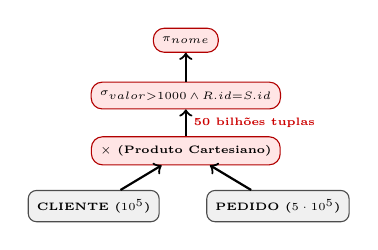
\begin{tikzpicture}[
    scale=0.78, every node/.style={transform shape},
    node/.style={rectangle, rounded corners=4pt, draw=red!70!black, fill=red!10, font=\bfseries\tiny, inner sep=4pt, align=center},
    base/.style={rectangle, rounded corners=3pt, draw=black!70, fill=black!6, font=\bfseries\tiny, inner sep=4pt}
  ]
    \node[node] (p) at (0, 2.7) {$\pi_{\text{nome}}$};
    \node[node] (s) at (0, 1.8) {$\sigma_{\text{valor} > 1000 \,\land\, R.\text{id} = S.\text{id}}$};
    \node[node] (x) at (0, 0.9) {$\times$ (Produto Cartesiano)};
    \node[base] (r) at (-1.5, 0.0) {CLIENTE ($10^5$)};
    \node[base] (srel) at (1.5, 0.0) {PEDIDO ($5 \cdot 10^5$)};

    \draw[->, thick] (r) -- (x);
    \draw[->, thick] (srel) -- (x);
    \draw[->, thick] (x) -- node[right, font=\tiny, text=red!80!black] {\textbf{50 bilhões tuplas}} (s);
    \draw[->, thick] (s) -- (p);
  \end{tikzpicture}
  \par\vspace{1mm}
  \tiny
  Consumo proibitivo de recursos temporários!
}{%
  \alert{Plano Otimizado com Push-Down}\par
  \vspace{1mm}
  \centering
  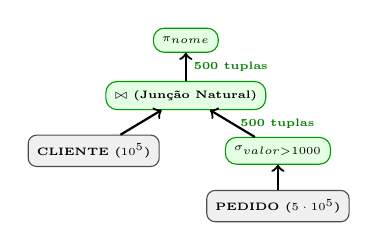
\begin{tikzpicture}[
    scale=0.78, every node/.style={transform shape},
    node/.style={rectangle, rounded corners=4pt, draw=green!60!black, fill=green!10, font=\bfseries\tiny, inner sep=4pt, align=center},
    base/.style={rectangle, rounded corners=3pt, draw=black!70, fill=black!6, font=\bfseries\tiny, inner sep=4pt}
  ]
    \node[node] (p) at (0, 2.7) {$\pi_{\text{nome}}$};
    \node[node] (j) at (0, 1.8) {$\bowtie$ (Junção Natural)};
    \node[base] (r) at (-1.5, 0.9) {CLIENTE ($10^5$)};
    \node[node] (s) at (1.5, 0.9) {$\sigma_{\text{valor} > 1000}$};
    \node[base] (srel) at (1.5, 0.0) {PEDIDO ($5 \cdot 10^5$)};

    \draw[->, thick] (srel) -- (s);
    \draw[->, thick] (s) -- node[right, font=\tiny, text=green!50!black] {\textbf{500 tuplas}} (j);
    \draw[->, thick] (r) -- (j);
    \draw[->, thick] (j) -- node[right, font=\tiny, text=green!50!black] {\textbf{500 tuplas}} (p);
  \end{tikzpicture}
  \par\vspace{1mm}
  \tiny
  Economia de 50.000.000.000 $\to$ 500 tuplas (Ganho de $100.000.000\times$)!
}
